\section{Evaluation}
\label{sec:evaluation}

\subsection{Hypotheses}
The primary hypothesis is that the motion of speckle patterns can be effectively visualized using a photodiode array. Additionally, it is hypothesized that the use of multiple lasers will influence the signal-to-noise ratio (SNR) of the measurements.

\subsection{Apparatus}
In setting up the evaluation, crucial parameters were carefully selected based on the technology utilized. 
The experimental setup involved the identification of dependent variables, with the use of a precision vibration table to facilitate controlled testing conditions.

\begin{figure}[t]
    \centering
    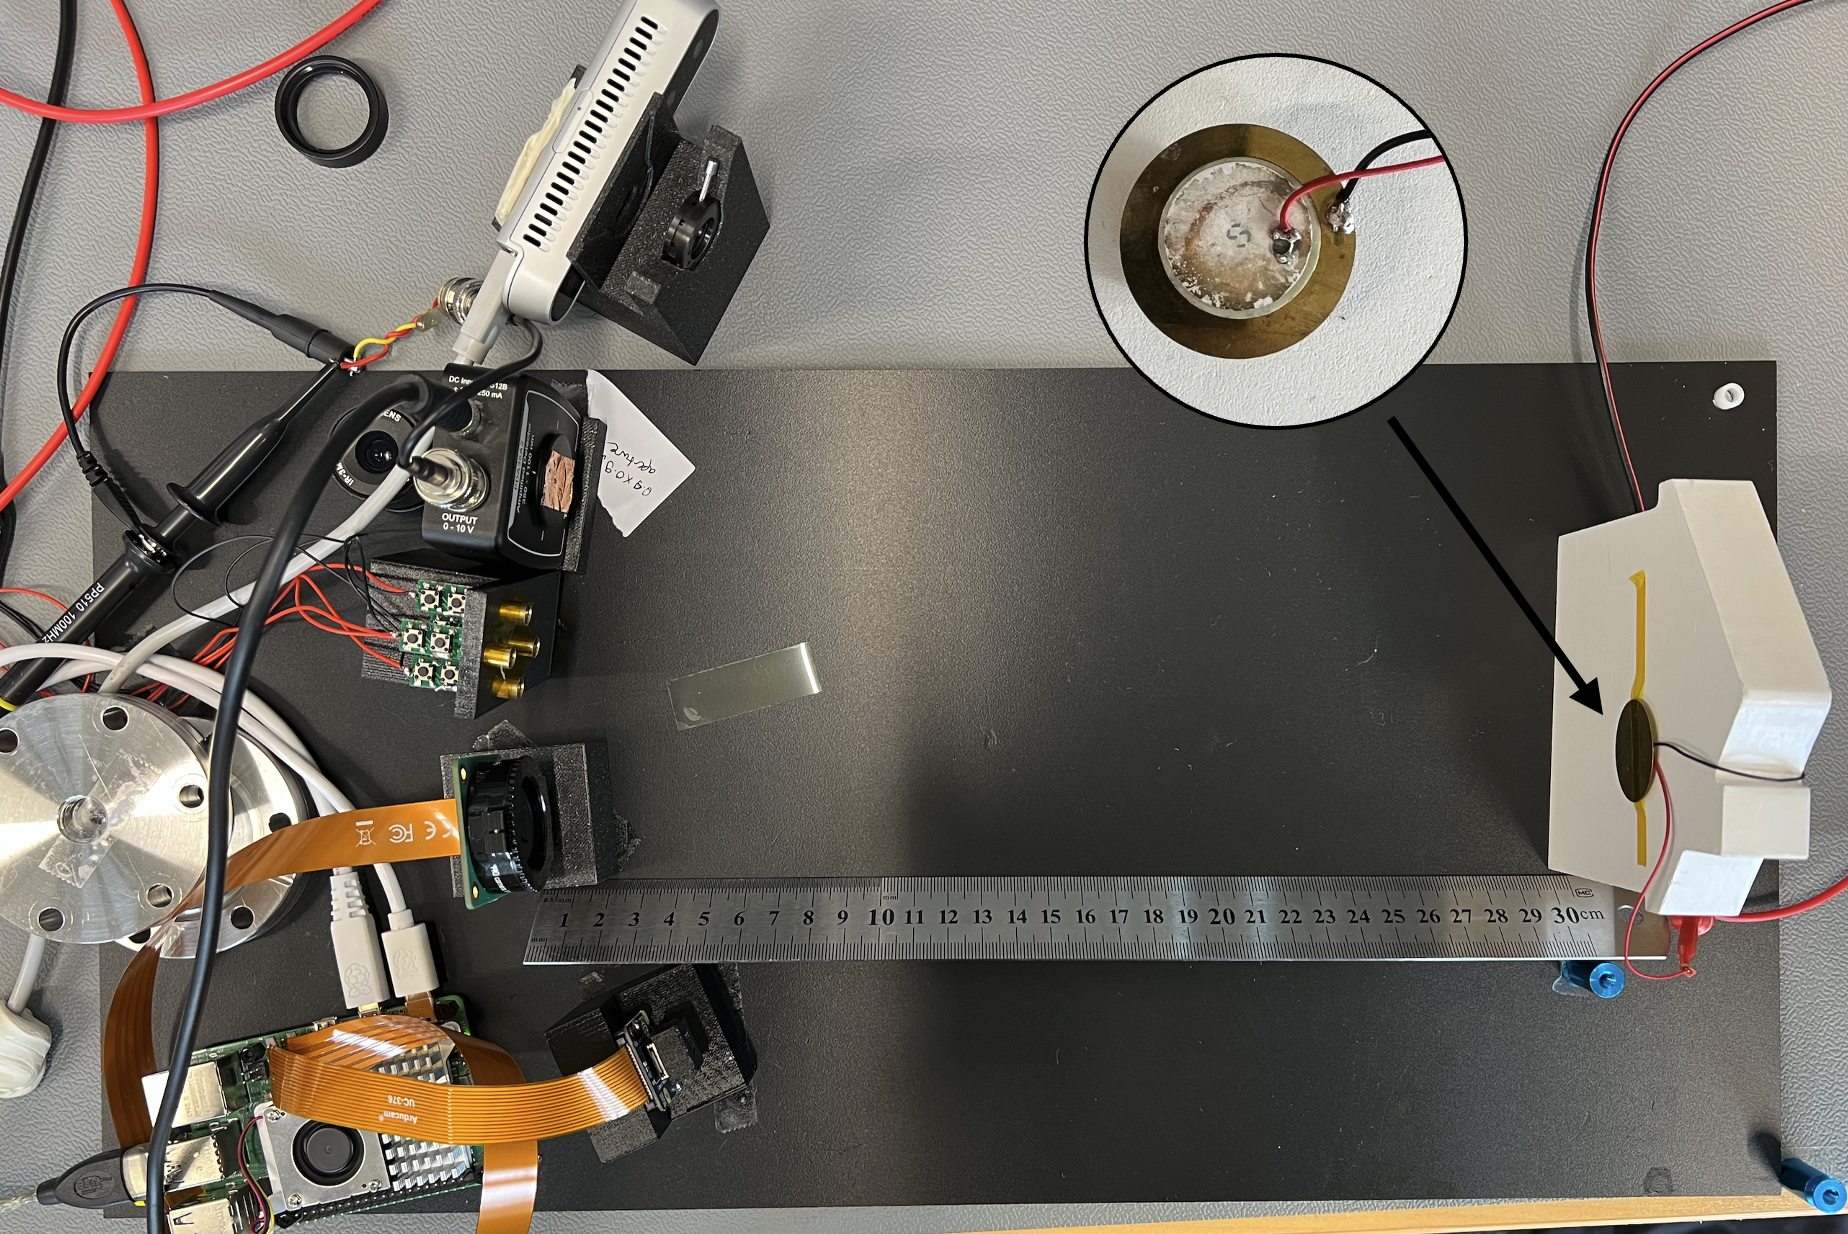
\includegraphics[width=\widthnarrow]{figures/eval/typical_setup.png}
    \caption{Photo of the standard experimental configuration.}
    \label{fig:setup}
\end{figure}

\subsection{Procedure}
The experimental procedure was designed to validate the performance of the printed circuit board (PCB) using a combination of detectors and lasers. 
We employed SPICE simulations to observe the Bode plot and transient response of the system, as illustrated in Figures~\ref{fig:bodeplot} and \ref{fig:transient}. 
The independent variables and experiment duration were rigorously controlled, with all measurements conducted in a light-controlled environment to mitigate external light interference. 
A comparative analysis was performed on the time-domain signals captured by multiple photodiodes. 
An infrared (IR) LED was incorporated to validate the hypothesis by ensuring that observed vibrations were not merely due to light interference.

\begin{figure}[t]
    \centering
    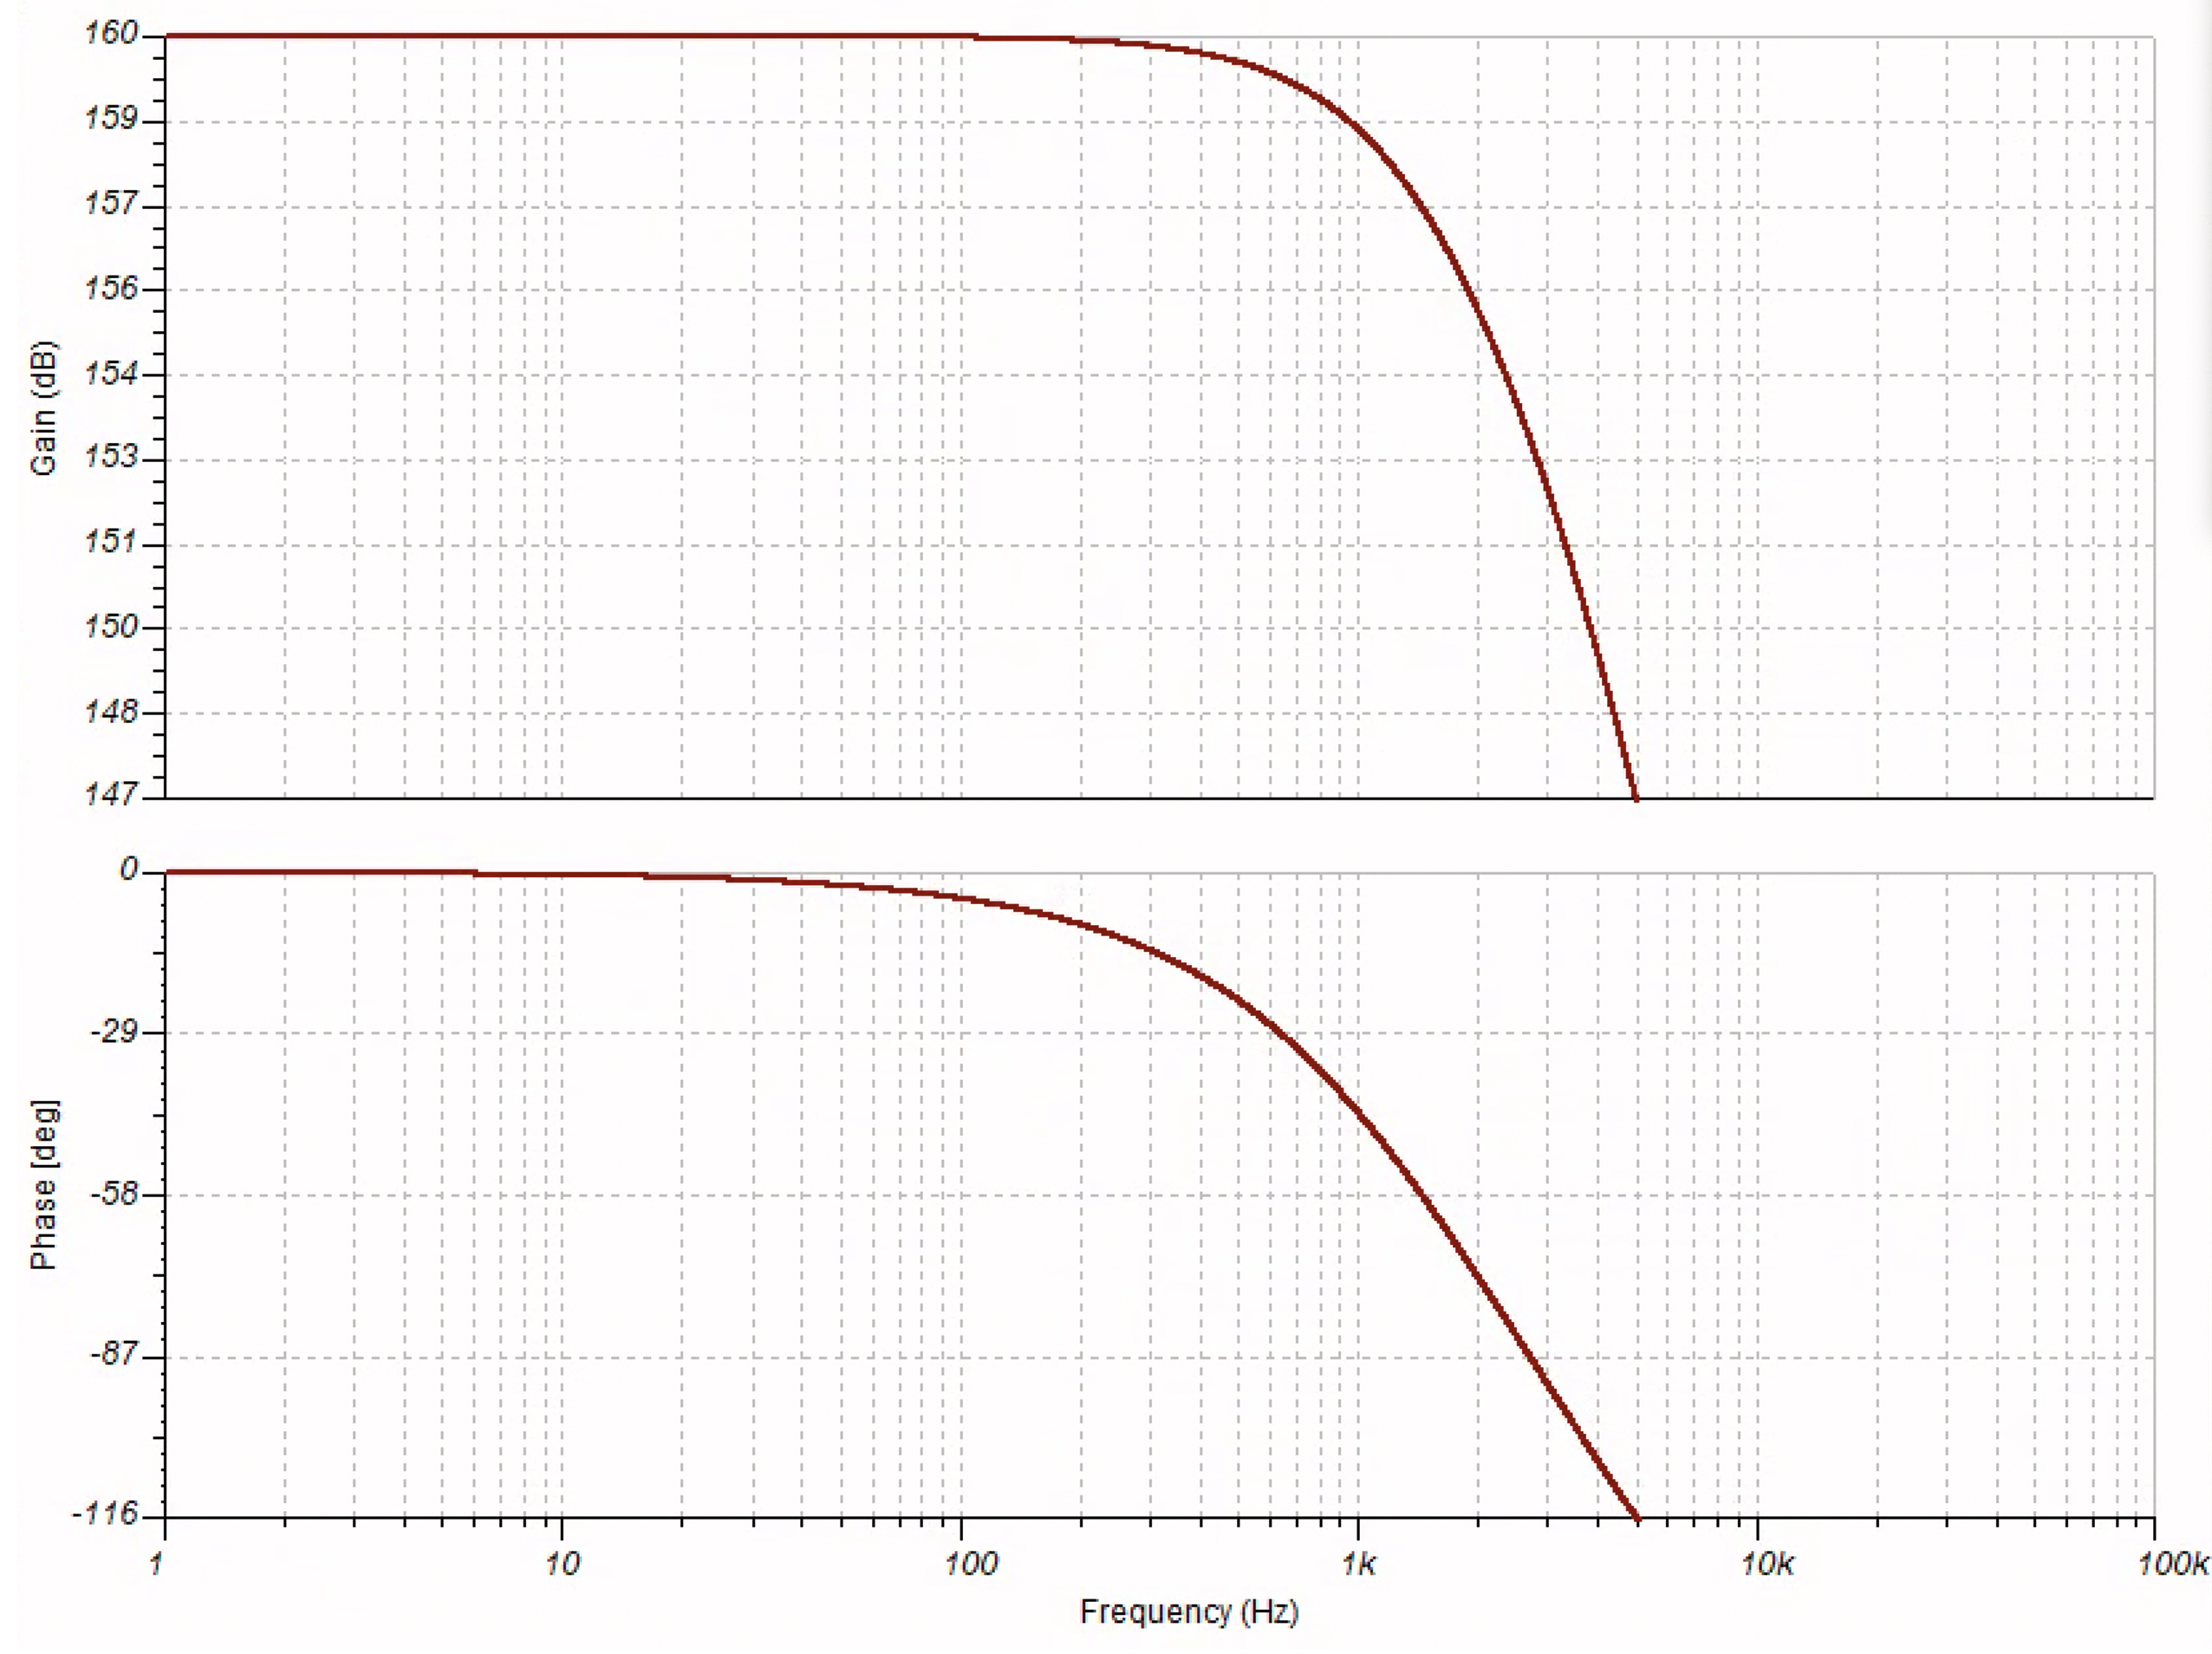
\includegraphics[width=\widthnarrow]{figures/eval/bode.png}
    \caption{The Bode plot demonstrates the frequency response of the evaluated circuit.}
    \label{fig:bodeplot}
\end{figure}

\begin{figure}[t]
    \centering
    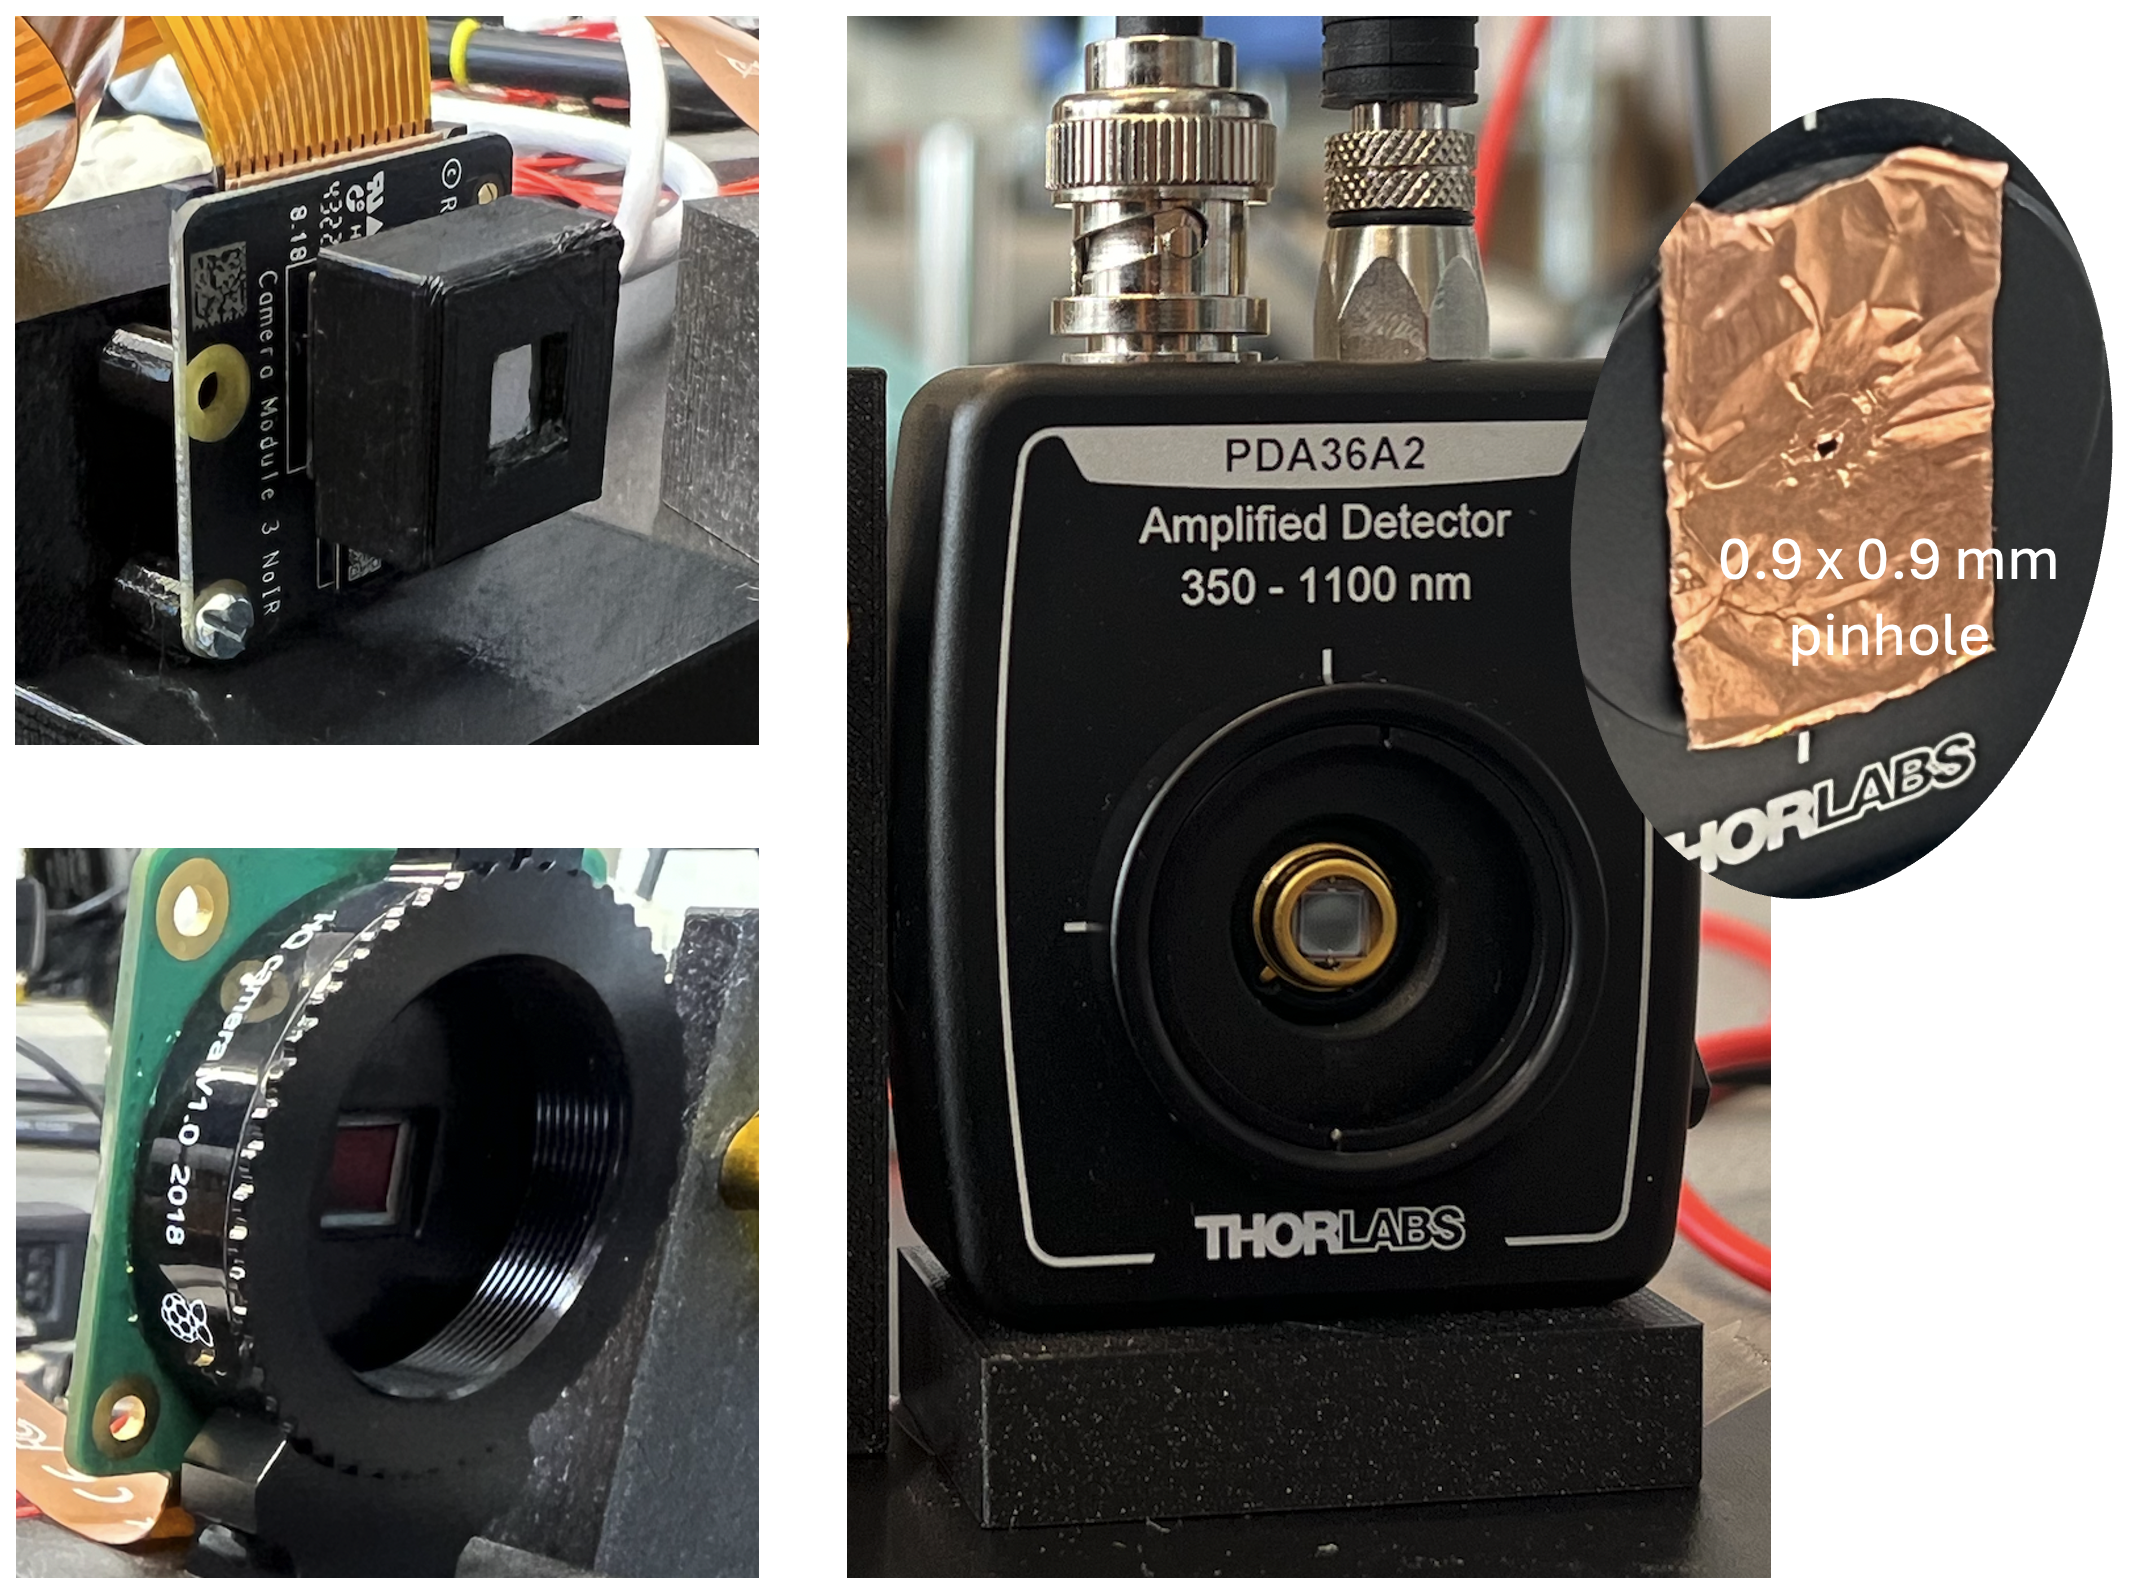
\includegraphics[width=\widthnarrow]{figures/eval/detectors.png}
    \caption{Setup of the photodiode array used for detection.}
    \label{fig:detectors}
\end{figure}


\begin{figure*}[t]
    \centering
    \includegraphics[width=\textwidth,height=1.8in]{figures/eval/speckles}
    \caption{Visualization of speckle patterns under different laser configurations.}
    \label{fig:speckles}
\end{figure*}

\begin{figure*}[t]
    \centering
    \includegraphics[width=\textwidth,height=1.8in]{figures/eval/lasers}
    \caption{Impact of multiple laser sources on SNR in the experimental setup.}
    \label{fig:lasers}
\end{figure*}

\begin{figure*}[t]
    \centering
    \includegraphics[width=\textwidth,height=1.8in]{figures/eval/transient}
    \caption{Transient response captured during SPICE simulation, highlighting system dynamics.}
    \label{fig:transient}
\end{figure*}